\subsection{CVSS-Vektor Selektion} \label{subsec:projektbericht-loesungsweg-cvss-selection}

Dank des Formats aus Kapitel \ref{subsec:projektbericht-loesungsweg-cvss-source-management} werden ab Generation 3 des Vulnerability Monitorings bei {\metaeffekt} $alle$ $Vektoren$ mitsamt ihren Quellen zu den gefundenen Schwachstellen während des Prozesses einfach in das Software-/Hardwareinventar aggregiert.
Im Gegensatz zur zweiten Generation, die diese Multiplizität ignorierte und eine pseudo-zufällige Auswahl durch ein \qt{First-Come-First-Serve}-Verfahren traf, soll das neue System eine gezielte Auswahl durch den Kunden ermöglichen.
Dieses Kapitel erläutert die Funktionsweise der CVSS-Vektor-Selektion.

Eine Vorbedingung zur Selektion ist natürlich die Sammlung aller relevanten Vektoren einer Schwachstelle, aus denen dann die Auswahl getroffen wird.
Dies umfasst Vektoren, die direkt mit der Schwachstelle verknüpft sind, aber auch solche, die von zugehörigen Security Advisories stammen.
Besondere Behandelung bei dieser Aggregation erfordern Vektoren mit spezifischen Anwendungsbedingungen, wie z.B.\ einige von Microsoft, die nur unter bestimmten Bedingungen anwendbar sind.
Zudem können projektinterne Bewertungsteams eigene Vektoren für eine Schwachstelle vergeben haben, die ebenfalls berücksichtigt werden müssen, und so weiter.

\ifshortenedReport
Zur Veranschaulichung wird der Prozess am Beispiel des Betriebssystems \qt{Windows 10 Pro} in Schaubild \ref{fig:cvss-selection-process-collection} dargestellt, das durch die Inventory Enrichment Pipeline läuft und mit den entsprechenden Schwachstellen und Security Advisories angereichert wird.
\else
Zur Veranschaulichung wird der Prozess am Beispiel des Betriebssystems \qt{Windows 10 Pro} dargestellt, das durch die Inventory Enrichment Pipeline, wie in Kapitel \ref{subsec:projektbericht-grundlagen-vulnerability-monitoring} beschrieben, läuft und mit den entsprechenden Schwachstellen und Security Advisories angereichert wird.
\fi
Nicht nur die Schwachstelle und die Security Advisories wurden mit CVSS-Vektoren versehen, sondern gab es auch mehrere Vektor-Modifikationen von manuellen Bewertungen als \qt{Assessment}-Vektoren.
Dieses Beispiel wird in Kapitel \ref{subsubsec:projektbericht-loesungsweg-cvss-selection-example} mit der eigentlichen Selektion der Vektoren fortgesetzt.

\begin{figure}[htbp] % here, top, bottom, separate page
    \centering
    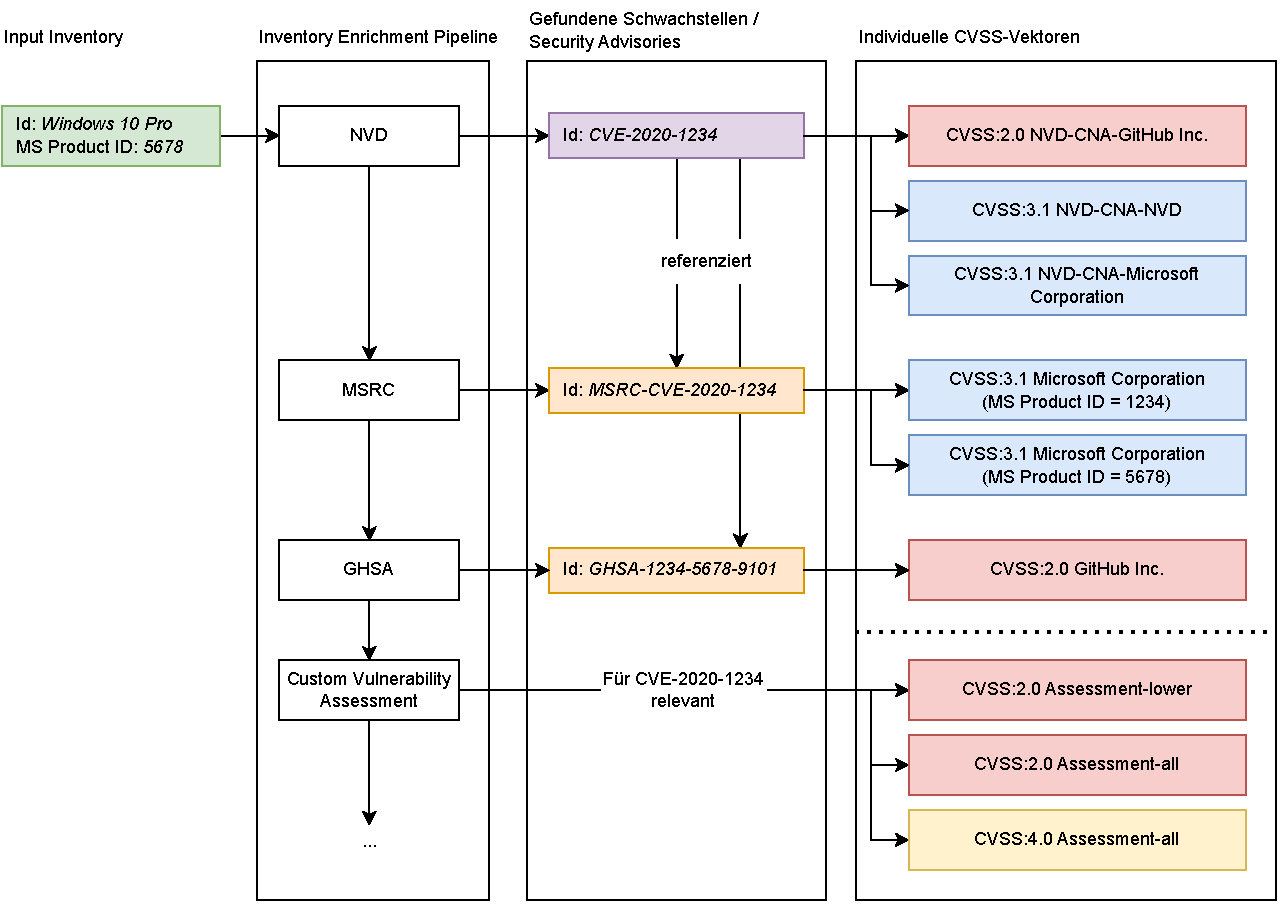
\includegraphics[width=1\textwidth, keepaspectratio]{res/grafiken/cvss-selection-process-collection}
    \caption{Beispiel: Initialer Zuordnungs- und Sammelungsschritt für Schwachstelldaten und CVSS-Vektoren}
    \label{fig:cvss-selection-process-collection}
\end{figure}

Nach der Zusammenführung aller CVSS-Vektoren beginnt die in zwei Teile gegliederte Phase der Selektion.
Da diese Selektoren wiederverwendbar und vollständig konfigurierbar sein müssen, können sie vollständig als JSON-Objekte ausgegeben und eingelesen werden.
Tatsächlich muss dieser Selektionsprozess in der Realität zweimal stattfinden, einmal mit einem \qt{initial} (der nur Vektoren externer Datenquellen berücksichtigt) und einmal mit einem \qt{context} Selektor (der auch \qt{assessment}-Vektoren aufnimmt), um den Kunden die Informationen Nachvollziehbar zu machen.
Die beiden hier kurz aufgeführten Schritte werden in den folgenden Unterkapiteln genauer erklärt.

\begin{enumerate}
    \item
    Der erste Schritt operiert pro Vektor-Version unabhängig voneinander und reduziert die Menge der Vektoren auf nur einen pro Version.
    Dieses Zwischenergebnis wird bereits von einigen Teilprozessen z.B.\ für die Darstellung in Radardiagrammen verwendet, um die Unterschiede zwischen den Versionen zu zeigen.
    \item
    Der zweite Schritt nimmt diese Menge aus bis zu drei Vektoren (im Moment: CVSS 2.0, 3.1, 4.0) und entscheidet, welche Version den effektiven Vektor für die Schwachstelle stellen soll.
    Dieser Schritt ist deutlich einfacher gestaltet, da dies nicht viel mehr als eine einzelne Regelentscheidung ist.
\end{enumerate}

\subsubsection{Schritt 1: Selektionsregeln} \label{subsubsec:projektbericht-loesungsweg-cvss-selection-rules-1}

Der erste Selektionsschritt lässt sich in drei Phasen unterteilen.
Der erste wählt durch vordefinierte Regeln relevante Vektoren aus und kombiniert diese durch in den Regeln festgelegten Methoden.
Die darauffolgenden beiden Schritte dienen zur Auswertung dieses kombinierten Vektors, um diesen eventuell zu manipulieren oder etwa in bestimmten Situationen gar keinen zurückzugeben.

In der folgenden Erklärung wird Bezug auf die Klasse \code{CvssSelector} genommen, welche reduziert auf wesentliche Attribute in Listing \ref{lst:cvss-selector-class-attributes} dargestellt wird.
Die Enumerationsdefinitionen, mit denen gewisse Aktionen signalisiert werden können, sind in Listing \ref{lst:cvss-selector-enum-definitions} zu finden.
Der vollständige Quellcode ist im \href{https://github.com/org-metaeffekt/metaeffekt-core/blob/24a26dd37ab6f9087e2fdc1b338857b404fa835e/libraries/ae-security/src/main/java/org/metaeffekt/core/security/cvss/processor/CvssSelector.java#L337}{[öffentlichen Repository]} einsehbar.
Eine wichtige Anforderung an das dahinterstehende Datenmodell ist die vollständige Serialisierbarkeit als JSON-Objekt, um eine identische Java-Objektstruktur rekonstruieren zu können.

\begin{lstlisting}[language=Java, label={lst:cvss-selector-class-attributes}, caption={CVSS-Selektor Klassen}, basicstyle=\scriptsize]
public class CvssSelector {
    // Die Attribute werden in diesen Unterkapiteln erklaert.
    List<CvssRule> rules; // 1.1
    List<SelectorStatsEvaluator> statsEvaluatorActions; // 1.2
    List<SelectorVectorEvaluator> selectorVectorEvaluators; // 1.3

    public static class CvssRule {
        SourceSelector sourceSelector;
        MergingMethod mergingMethod;
        List<SelectorStatsCollector> statsCollectors;
        List<SelectorVectorEvaluator> vectorEvaluators;
    }
    public static class SourceSelector {
        List<SourceSelectorEntry> preferredSources;
    }
    public static class SourceSelectorEntry {
        List<SourceSelectorEntryEntry<CvssEntity>> hostingEntities;
        List<SourceSelectorEntryEntry<CvssEntity>> issuingEntities;
        List<SourceSelectorEntryEntry<CvssIssuingEntityRole>> issuingEntityRoles;
    }
    public static class SourceSelectorEntryEntry<T extends CvssSource.EntityNameProvider> {
        T value;
        boolean inverted;
    }
    public static class SelectorStatsCollector {
        String attributeName;
        StatsCollectorProvider provider;
        StatsCollectorSetType setType;
    }
    public static class SelectorVectorEvaluator {
        // operations are combined using AND
        // individual operations can be inverted by setting value to true
        Map<VectorEvaluatorOperation, Boolean> operations;
        EvaluatorAction action;
    }
    public static class SelectorStatsEvaluator {
        String attributeName;
        StatsEvaluatorOperation comparator;
        EvaluatorAction action;
        Integer comparisonValue;
    }
}
\end{lstlisting}

\begin{lstlisting}[language=Java, label={lst:cvss-selector-enum-definitions}, caption={CVSS-Selektor Enumerations}, basicstyle=\scriptsize]
public enum MergingMethod           { ALL, LOWER, HIGHER, OVERWRITE            }
public enum StatsCollectorProvider  { PRESENCE, ABSENCE, APPLIED_PARTS_COUNT   }
public enum StatsCollectorSetType   { ADD, SUBTRACT, SET, MAX, MIN             }
public enum EvaluatorAction         { FAIL, RETURN_NULL, SKIP, RETURN_PREVIOUS }
public enum StatsEvaluatorOperation {
    EQUAL, SMALLER, SMALLER_OR_EQUAL, GREATER, GREATER_OR_EQUAL
}
public enum VectorEvaluatorOperation {
    IS_NULL, IS_BASE_FULLY_DEFINED, IS_BASE_PARTIALLY_DEFINED, IS_ENVIRONMENTAL_PARTIALLY_DEFINED,
    IS_TEMPORAL_PARTIALLY_DEFINED, IS_THREAT_PARTIALLY_DEFINED
}
\end{lstlisting}

\paragraph{Schritt 1.1: Regeln zur Vektor-Selektion und -Kombination} \label{par:projektbericht-loesungsweg-cvss-selection-rules-1-1}

Für die Auswahl und Kombination der endgültigen Vektoren definiert der Benutzer eine Reihe von Regeln.
Die Abfolge an Regeln kann man sich als Pipeline vorstellen, in der jeweils ein Vektor ausgewählt und mit dem vorherigen kombiniert wird.
Der Startvektor ist einfach ein leerer Vektor, der nach und nach gefüllt wird.
Die Regeln, repräsentiert durch \code{SourceSelectorEntry} in der Klasse \code{SourceSelector}, nutzen die im Kapitel \ref{subsec:projektbericht-loesungsweg-cvss-source-management} eingeführte Vektor-Quellennotation zur Spezifizierung des auszuwählenden Vektors.
Durch Angabe von Hosting- und Issuing-Entities (sowie einer Issuing Role), wird der erste zutreffende Vektor aus der aggregierten Liste gewählt, wobei Sonderwerte wie \qt{*} für beliebige Werte und \qt{null} für leere Werte verwendet werden können.
Diese können optional invertiert werden, um komplexere Abfragen zu ermöglichen.
Da der erste erfolgreiche Vektor-Match zurückgegeben wird, können so Fallback-Strategien definiert werden.

Die \code{MergingMethod} in der Regel legt dann fest, wie der gefundene Vektor mit dem vorherigen kombiniert wird.
\code{ALL} übernimmt alle Metriken des neuen Vektors, während \code{HIGHER} und \code{LOWER} den Score nur dann ändern, wenn der resultierende Vektor einen höheren bzw.\ niedrigeren Score erzeugt.
\code{OVERWRITE} ersetzt den vorherigen Vektor vollständig.
Mithilfe des \code{SelectorStatsCollector} werden verschiedene Statistiken in benutzerdefinierten Variablen für die Auswertung in Schritt 1.2 gesammelt.
Ein \qt{Statistics Collector} kann beispielsweise aufzeichnen, ob ein Vektor durch eine bestimmte Regel gefunden wurde oder bei den Methoden \code{HIGHER} und \code{LOWER} wie viele Metriken konkret angewendet wurden.
Diese Variablen bleiben bis zur Auswertung in Schritt 1.2 erhalten.

Jede Regel kann abschließend mit dem \code{SelectorVectorEvaluator} weitere (optional invertierbare) Überprüfungen durchführen.
Diese können Aktionen über \code{EvaluatorAction} auslösen, wie den Prozess abzubrechen, einen leeren Vektor zurückzugeben, eine Regel zu überspringen oder an der vorherigen Regel festzuhalten.

% Horizontal is this instance, vertical is the parameter.
% |       | ANY | value | null |
% |-------|-----|-------|------|
% | ANY   | Y   | Y     | Y    |
% | value | Y   | ==    | N    |
% | null  | N   | N     | Y    |

\paragraph{Schritt 1.2: Statistics Evaluators (Statistik-Auswerter)}

Nachdem in Schritt 1.1 ein einziger, kombinierter Vektor erstellt wurde, können optional bestimmte \qt{Statistics Collectors} mittels nutzerdefinierten \code{SelectorStatsEvaluator} ausgewertet werden.
Es stehen typische numerische Vergleichsoperationen wie größer, kleiner, gleich, \dots\ zur Verfügung, um Aktionen über die bereits genannten \code{EvaluatorAction} zu initiieren.
Ein Beispiel wäre, dass ein Vektor nur dann akzeptiert wird, wenn er mindestens einen Vektor einer gewissen Quelle enthält, im eigentlichen Beispiel wird darauf allerdings noch genauer eingegangen.

\paragraph{Schritt 1.3: Vector Evaluators}

Letzte Überprüfungen am Ergebnisvektor erfolgen erneut über \code{SelectorVectorEvaluator}, wobei Aktionen durch \code{EvaluatorAction} ausgelöst werden können, ähnlich wie in Schritt 1.1 beschrieben.
Die Operationen sind hier auf die Vektor-Metadaten beschränkt, wie z.B.\ ob der Basis-Vektor vollständig definiert ist oder nicht.
Dieser gesamte Prozess wird für jede Vektor-Version (2.0, 3.1, 4.0) einmal durchgeführt, mit jeweils zwei Selektoren (initial, context), was zu einer recht großen Auswahl von bis zu sechs Vektoren führen kann.

\subsubsection{Schritt 2: Versions-Selektionsregeln} \label{subsubsec:projektbericht-loesungsweg-cvss-selection-rules-2}

Dieser Schritt ist einfacher als der erste, da nur entschieden werden muss, welche Vektor-Version den effektiven Vektor stellen soll.
Es kann hier eine Liste an \code{CvssScoreVersionSelectionPolicy}-Werten verwendet werden, die in Listing \ref{lst:cvss-selector-version-selector} definiert sind, die nach einer Fallback-Strategie wählen.
Die am häufigsten verwendeten Optionen sind \code{LATEST} und \code{HIGHEST}.

\begin{lstlisting}[language=Java, label={lst:cvss-selector-version-selector}, caption={Gültige Werte für die Versions-Selektion}]
public enum CvssScoreVersionSelectionPolicy {
    HIGHEST, LOWEST, LATEST, OLDEST, V2, V3, V4
}
\end{lstlisting}

Mit Anwenden dieser Schritte ist der Selektionsprozess abgeschlossen.
Im nächsten Abschnitt wird dieser Prozess anhand eines Beispiels veranschaulicht.

\newpage
\subsubsection{Beispiel zur Vektor-Selektion} \label{subsubsec:projektbericht-loesungsweg-cvss-selection-example}

Das Beispiel, begonnen unter Kapitel \ref{subsec:projektbericht-loesungsweg-cvss-selection} im Schaubild \ref{fig:cvss-selection-process-collection}, wird hier mit den aggregierten Vektoren fortgeführt.
Um die Selektion durchzuführen, müssen zwei Selektoren für initial und context definiert werden, \href{https://github.com/org-metaeffekt/metaeffekt-core/blob/1f0a1f6ac5e8343e10ea182794faf534bdfb3310/libraries/ae-inventory-processor/src/main/java/org/metaeffekt/core/inventory/processor/report/configuration/CentralSecurityPolicyConfiguration.java\#L568}{[genommen aus Produktionscode]}, die dank einer \code{CvssSelector.explain()}-Methode als menschenlesbarer Text dargestellt werden können.

\paragraph{Beispiel, CVSS-Selektor \qt{initial}} \label{par:projektbericht-loesungsweg-cvss-selection-example-selector-initial}

\

\noindent The CVSS Selector contains 1 rule that will be applied in the following order:
\begin{enumerate}[noitemsep]
    \setlist{nolistsep}
    \item The first matching vector is selected: [NVD-CNA-NVD], [Microsoft Corporation-*-*], [NVD-CNA-Microsoft Corporation], [GitHub, Inc.-*-*], [NVD-CNA-GitHub, Inc.], [NVD-*-*], [CERT-SEI-*-*], [not:Assessment-*-*]. From the selected vector, all vector components are applied to the resulting vector.
\end{enumerate}

\paragraph{Beispiel, CVSS-Selektor \qt{context}} \label{par:projektbericht-loesungsweg-cvss-selection-example-selector-context}

\

\noindent The CVSS Selector contains 4 rules that will be applied in the following order:
\begin{enumerate}[noitemsep]
    \setlist{nolistsep}
    \item The first matching vector is selected: [NVD-CNA-NVD], [Microsoft Corporation-*-*], [NVD-CNA-Microsoft Corporation], [GitHub, Inc.-*-*], [NVD-CNA-GitHub, Inc.], [NVD-*-*], [CERT-SEI-*-*], [not:Assessment-*-*]. From the selected vector, all vector components are applied to the resulting vector.
    \item If present, the [Assessment-*-all] vector is selected. From the selected vector, all vector components are applied to the resulting vector. The following 1 statistics collector will also be applied to the selected vector:
    \begin{itemize}[noitemsep]
        \item If a vector is returned from the selection, 1 is added to the stats collector attribute [assessment].
    \end{itemize}
    \item If present, the [Assessment-*-lower] vector is selected. From the selected vector, only vector components that lead to a lower or equal score on the resulting vector are applied. The following 1 statistics collector will also be applied to the selected vector:
    \begin{itemize}[noitemsep]
        \item If a vector is returned from the selection, 1 is added to the stats collector attribute [assessment].
    \end{itemize}
    \item If present, the [Assessment-*-higher] vector is selected. From the selected vector, only vector components that lead to a higher or equal score on the resulting vector are applied. The following 1 statistics collector will also be applied to the selected vector:
    \begin{itemize}[noitemsep]
        \item If a vector is returned from the selection, 1 is added to the stats collector attribute [assessment].
    \end{itemize}
\end{enumerate}

\noindent After finishing the CVSS selection, 1 statistics evaluator will be applied to the resulting vector:
\begin{itemize}[noitemsep]
    \setlist{nolistsep}
    \item If the stats collector attribute [assessment] is equal to 0, then no vector is returned.
\end{itemize}
Additionally, 1 vector evaluator will be applied to the resulting vector:
\begin{itemize}[noitemsep]
    \setlist{nolistsep}
    \item If the resulting vector is not base fully defined, then no vector is returned.
\end{itemize}

\newpage
\paragraph{Beispiel, Schritt 1: Aggregieren der Vektoren} \label{par:projektbericht-loesungsweg-cvss-selection-example-step-1}

Dieser Abschnitt bezieht sich auf Schaubild \ref{fig:cvss-selection-process-selection-1}.
Wie im Hauptteil erklärt, wird als Ausgangspunkt für die Selektionsschritte eine Sammlung von Vektoren benötigt.
In diesem Beispiel werden die Vektoren der Schwachstelle \qt{CVE-2020-1234} selbst und die dazugehörigen manuellen Bewertungen (\qt{Assessments}) auf jeden Fall berücksichtigt.
Bei dem Security Advisory von Microsoft mit \qt{MSRC-CVE-2020-1234} können allerdings nicht alle Vektoren übernommen werden, denn jeder Vektor gilt nur der nur für bestimmte Produkt-IDs.
Unsere Produkt-ID ist \qt{5678}, daher wird der Vektor mit der ID \qt{MS Product ID 1234} ausgeschlossen.

\begin{figure}[htbp] % here, top, bottom, separate page
    \centering
    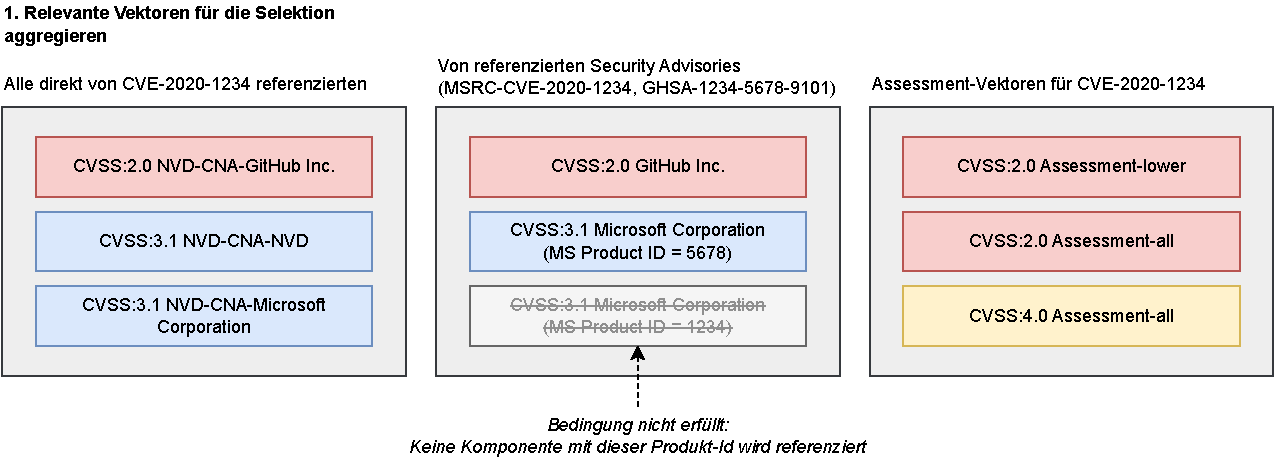
\includegraphics[width=1\textwidth, keepaspectratio]{res/grafiken/cvss-selection-process-selection-1}
    \caption{Aggregierung der CVSS-Vektoren}
    \label{fig:cvss-selection-process-selection-1}
\end{figure}

\paragraph{Beispiel, Schritt 2: Anwenden der CVSS-Selektoren} \label{par:projektbericht-loesungsweg-cvss-selection-example-step-2}

\begin{figure}[htbp] % here, top, bottom, separate page
    \centering
    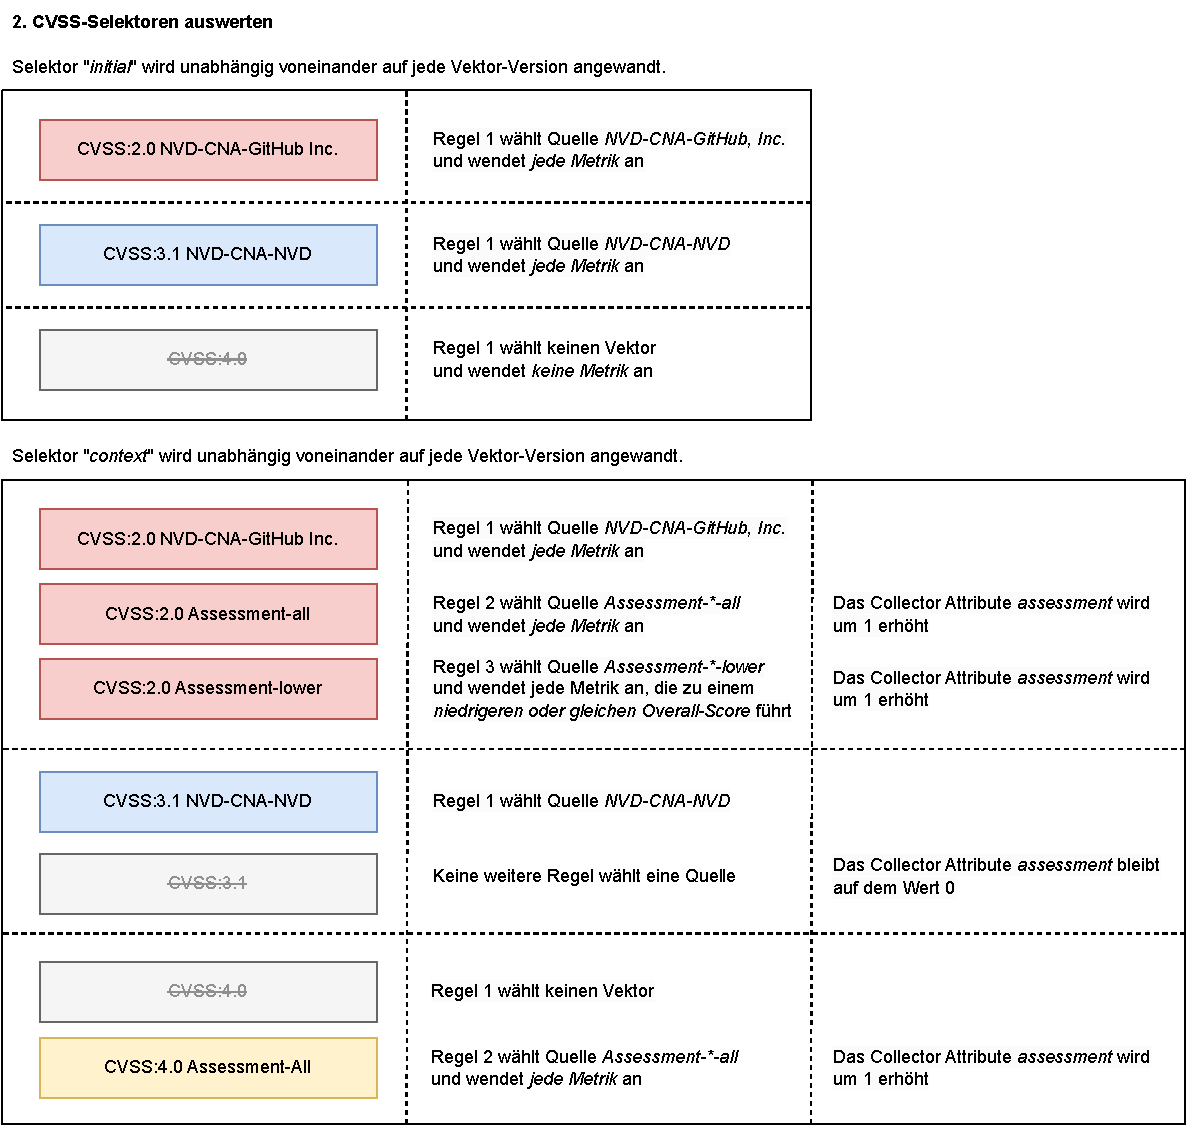
\includegraphics[width=1\textwidth, keepaspectratio]{res/grafiken/cvss-selection-process-selection-2}
    \caption{Auswerten der CVSS-Selektoren}
    \label{fig:cvss-selection-process-selection-2}
\end{figure}

\begin{figure}[htbp] % here, top, bottom, separate page
    \centering
    \includegraphics[width=1\textwidth, keepaspectratio]{res/grafiken/cvss-selection-process-selection-3}
    \caption{Ergebnisse der CVSS-Selektion}
    \label{fig:cvss-selection-process-selection-3}
\end{figure}

Die Schaubilder \ref{fig:cvss-selection-process-selection-2} und \ref{fig:cvss-selection-process-selection-3} illustrieren diesen Schritt.
Auf die gesammelten Vektoren werden nun die oben genannten Selektoren angewendet.
Der \qt{initial}-Selektor wählt die erste passende Quelle pro Version aus der Liste der Regeln aus, wobei außer für CVSS:4.0 (besitzt keine nicht-Assessment-Vektoren) stets genau ein Vektor zurückgegeben wird.
Der \qt{context}-Selektor startet mit denselben initialen Vektoren, findet jedoch für CVSS:2.0 durch weitere Regeln zusätzliche Vektoren, die gemäß den festgelegten Regeln (alle Metriken oder nur \qt{lower}) angewendet werden.
Für CVSS:4.0 trägt ausschließlich ein Assessment-Vektor bei, nicht durch Regel 1.
Das System vermerkt zudem, ob mindestens ein Assessment-Vektor vorhanden war, was nur bei CVSS:3.1 nicht der Fall ist.
Daraus folgt, wie in Schaubild \ref{fig:cvss-selection-process-selection-3} dargestellt, dass für CVSS:2.0 ein kombinierter und für CVSS:4.0 der Assessment-Vektor ausgewählt wurde, während für CVSS:3.1 kein Vektor zurückgegeben wurde, da der Statistics Evaluator das \qt{assessment}-Attribut mit negativem Ergebnis überprüft hat.

\paragraph{Beispiel, Schritt 3: Anwenden der Versions-Selektion} \label{par:projektbericht-loesungsweg-cvss-selection-example-step-4}

Dieser Abschnitt bezieht sich auf Schaubild \ref{fig:cvss-selection-process-selection-4}.
Nun können die verbleibenden Vektoren auf einen einzigen je \qt{initial} und \qt{context} durch den Versions-Seletor reduziert werden.
Es wird die Regel \code{LATEST} angewendet, sodass die neueste Vektor-Version ausgewählt wird.
Diese Vektoren stehen nun für weitere Verarbeitungsschritte zur Verfügung.

\begin{figure}[htbp] % here, top, bottom, separate page
    \centering
    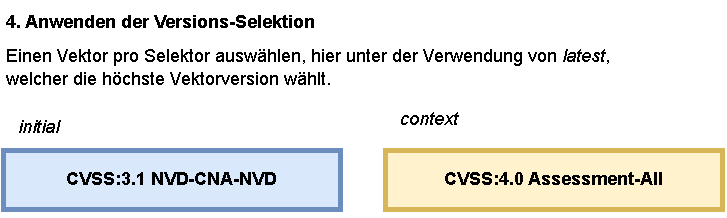
\includegraphics[width=0.7\textwidth, keepaspectratio]{res/grafiken/cvss-selection-process-selection-4}
    \caption{Anwenden der Versions-Selektion}
    \label{fig:cvss-selection-process-selection-4}
\end{figure}
